% =========================================================================== %

\begin{frame}[t,plain]
\titlepage
\end{frame}

% =========================================================================== %

\begin{frame}{Recap}
%
\begin{columns}[T]
\column{.5\linewidth}
\begin{itemize}
\item Datentypen Umwandeln
	\begin{itemize}
	\item Datentyp-Bezeichner als Funktion, \zB \inPy{int("3")}
	\item Informationsverlust möglich: \\
		\inPy{int(3.1)} ~\thus~ \inPy{3}
	\end{itemize}
\item Formatierte Texte
	\begin{itemize}
	\item \inPy{f"Text {Ausdruck:Format}"}
	\item Vor- und Nachkommastellen, Zentrieren, ...
	\item Bei Bedarf nachschlagen
	\end{itemize}
\end{itemize}
%
\column{.5\linewidth}
\begin{itemize}
\item Wahrheitswerte
	\begin{itemize}
	\item Typ \inPy{bool} speichert \inPy{True} oder \inPy{False}
	\item Vergleichsoperatoren (\inPy{==}, \inPy{>=}, ...)
	\end{itemize}
\item Bedingte Ausführung
	\begin{itemize}
	\item Mit \inPy{if}: Eingerückter Code
	\item \inPy{elif}: Alternativ-Bedingungen
	\item \inPy{else}: Sonst-Code
	\item Prüfung von oben nach unten
	\item Nur erster Treffer wird ausgeführt
	\item Kann verschachtelt werden
	\end{itemize}
\end{itemize}
\end{columns}
%
\begin{center}
	\emph{Noch Fragen?}
\end{center}
%
\end{frame}

% =========================================================================== %

\begin{frame}[fragile]{Durch die Übung inspirierte Frage}
%
\begin{center}
	\begin{Large}
	\emph{Ist es möglich, Gleichungen eingeben und auswerten zu lassen?}
	\end{Large}
\end{center}
%
\begin{itemize}
\item Ja, aber eine gefährliche. (Oder eine ungefährliche, sehr komplizierte)
\item Befehl \inPy{eval} nimmt einen String, und führt diesen als Python-Code aus.
\item Ergebnis dieser Ausführung als Rückgabewert: \inPy{result = eval("x** 2 + 5")}
\item String kann \emph{beliebigen} Python-Code enthalten, auch schadhaften Code.
\end{itemize}
%
\begin{warnbox}[Code Injection und \texttt{eval}]
Eingaben durch den User sind immer eine Gefahrenquelle, sowohl durch Versehen als auch durch boshafte Absicht.\\
Sie sollten \emph{immer} auf Sinnhaftigkeit getestet und möglichst stark beschränkt werden.
\end{warnbox}
%
\end{frame}

% =========================================================================== %

\begin{frame}{xkcd: Exploits of a Mom}
%
\begin{center}
	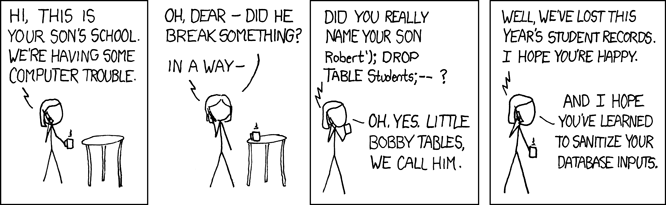
\includegraphics[width=.8\linewidth]{./gfx/xkcd-codeInjection}\\
	\vspace{3pt}
	
	\scriptsize \emph{Her daughter is named Help I'm trapped in a driver's license factory.}
	\vspace{6pt}\\
	
	Source: \url{https://xkcd.com/327/}
\end{center}
%
\end{frame}

% =========================================================================== %

\begin{frame}{Kapitel 3}
%
\begin{itemize}
\item Module
	\begin{itemize}
	\item Sammlung von Routinen
	\item Laden und Funktionen nutzen
	\end{itemize}
\end{itemize}
%
\end{frame}

% =========================================================================== %

\begin{frame}[fragile]
%
\begin{columns}
\column{.5\linewidth}
\begin{Large}
Module Laden
\vspace{6pt}
\end{Large}
\begin{itemize}
\item Python-Sprachumfang nicht sehr groß (nur 33 Schlüsselworte)
\item Aus diesen können jedoch \enquote{komplexere Maschinen} zusammengesetzt werden
\item Braucht Speicherplatz und Zeit zum Laden
\item Nie alle Konstruktionen gleichzeitig nötig
\item[\Thus] Laden \enquote{on demand}
\item[\Thus] Befehl \inPy{import}
\item Modul: Sammlung von vorgefertigten Lösungen
\end{itemize}
%
\column{.5\linewidth}
\begin{codebox}[Syntax: \texttt{import}]
\begin{minted}[fontsize=\scriptsize]{python}
import Modulname
\end{minted}
\end{codebox}
\begin{itemize}
\item Beispiel: \texttt{math}: Gängige mathematische Funktionen (exp, sin, sqrt, ...)
\item Beispiel: \texttt{cmath}: Selbe Funktionen für komplexe Zahlen
\item Lädt Code in den Arbeitsspeicher
\item Code kommt...
	\begin{itemize}
	\item entweder aus dem aktuellen Arbeitsverzeichnis
	\item oder aus einem Standard-Ordner
	\end{itemize}
\end{itemize}
\end{columns}
%
\end{frame}

% =========================================================================== %

\begin{frame}[fragile]{Funktionen aus Modulen benutzen}
%
\begin{columns}
\column{.5\linewidth}
\begin{itemize}
\item Zwei Module können gleichnamige Funktionen enthalten
\item Daher: \inPy{Modulname.Objekt}
\item Objekt: Funktion oder Konstante
\end{itemize}
%
\column{.5\linewidth}
\begin{itemize}
\item \texttt{sin} -- Sinus
\item \texttt{pi} -- $\pi$
\item Jeweils in reellwertiger (\texttt{math}) und komplexer (\texttt{cmath}) Form 
\end{itemize}
\end{columns}
%
\begin{tcbraster}[raster columns=2,
                  raster equal height,
                  nobeforeafter,
                  raster column skip=0.5cm]
\begin{codebox}[Beispiel: Sinus aus zwei Modulen]
\begin{minted}[fontsize=\scriptsize]{python}
import cmath
import math

print( math. sin( math.pi / 2) )
print( cmath.sin(cmath.pi / 2) )
\end{minted}
\end{codebox}
%
\begin{cmdbox}[Ausgabe]
\begin{minted}[fontsize=\scriptsize]{text}
1.0
(1+0j)
\end{minted}
\end{cmdbox}
\end{tcbraster}
%
\end{frame}

% =========================================================================== %

\begin{frame}{Kapitel 4}
%
\begin{itemize}
\item Datenstrukturen
	\begin{itemize}
	\item Speichermodell
	\item Mutable vs. Immutable
	\item \inPy{list}s
	\item Slices
	\item Methoden und spezielle Funktionen
	\end{itemize}
\end{itemize}
%
\end{frame}

% =========================================================================== %

\begin{frame}[fragile]{Datencontainer -- \inPy{list}s}
%
\begin{columns}
\column{.5\linewidth}
\begin{itemize}
\item Bisher: Nur eine einzige Informationseinheit gleichzeitig \enquote{in der Hand} (einzelne Zahlen)
\item Oft nötig: \emph{Listen} von Werten
\item Neuer Datentyp: \inPy{list}
\item Zusammenfassung von beliebig vielen Werten beliebigen Typs
\item Unterscheidung durch einen \emph{Index} (\enquote{Zeilennummer in der Liste})
\item \emph{Indices beginnen bei 0!}
\end{itemize}
%
\column{.5\linewidth}
\begin{codebox}[Syntax: Listen Erstellen]
\begin{minted}[fontsize=\scriptsize]{python}
Variable = [Element1, Element2, ...]
\end{minted}
\end{codebox}
%
\begin{codebox}[Syntax: Listenelement Verändern]
\begin{minted}[fontsize=\scriptsize]{python}
Variable[Index] = neuerWert
\end{minted}
\end{codebox}
%
\begin{codebox}[Syntax: Listenelement Lesen]
\begin{minted}[fontsize=\scriptsize]{python}
print(Variable[Index])
\end{minted}
\end{codebox}
\end{columns}
%
\end{frame}

% =========================================================================== %

\begin{frame}[fragile]
%
\begin{tcbraster}[raster columns=2,
                  raster equal height,
                  nobeforeafter,
                  raster column skip=0.5cm]
\begin{codebox}[Beispiel: Listen]
\begin{minted}[fontsize=\scriptsize, linenos]{python}
values = [1, 2, 3, 
          "anderer Datentyp", 
          ["eine", "Liste", 
           "in", "der", "Liste"]
         ]
print(values)
print(values[0])
print(values[4])
\end{minted}
\end{codebox}
%
\begin{cmdbox}[Ausgabe]
\begin{minted}[fontsize=\scriptsize]{text}
[1, 2, 3, 'anderer Datentyp', ['eine', 
 'Liste', 'in', 'der', 'Liste']]
1
['eine', 'Liste', 'in', 'der', 'Liste']
\end{minted}
\end{cmdbox}
\end{tcbraster}
%
\end{frame}

% =========================================================================== %

\begin{frame}[fragile]
%
\begin{columns}[t]
\column{.5\linewidth}
\begin{Large}
{Indices: Erweiterte Features}
\vspace{6pt}
\end{Large}
\begin{itemize}
\item Negative Indices: \enquote{von hinten herein zählen}
	\begin{itemize}
	\item \texttt{Variable[-1]}: Letztes Element der Liste
	\end{itemize}
\item \enquote{Slices}
	\begin{itemize}
	\item Ausschnitte einer Liste auswählen
	\item Logik \enquote{Start : Stop : Schrittweite}
	\item Teile können ausgelassen werden
	\item \texttt{Variable[Start:Stop]}: Alles zwischen \emph{einschließlich} Index \texttt{Start} und \emph{ausschließlich} Index \texttt{Stop}
	\item \texttt{Variable[Start::n]}: Jeder \texttt{n}-te Wert, beginnend bei Index \texttt{Start}
	\end{itemize}
\end{itemize}
%
\column{.5\linewidth}
\begin{codebox}[Beispiel: Index-Features]
\begin{minted}[fontsize=\scriptsize, linenos]{python}
myList = [0,1,2,3,4,5,6,7,8,9,10]
print(myList[-1], myList[-2])
print(myList[0:-1:2])
print(myList[2::2])
print(myList[::2])
print(myList[:5])
\end{minted}
\end{codebox}
%
\begin{cmdbox}[Ausgabe]
\begin{minted}[fontsize=\scriptsize]{text}
10 9
[0, 2, 4, 6, 8]
[2, 4, 6, 8, 10]
[0, 2, 4, 6, 8, 10]
[0, 1, 2, 3, 4]
\end{minted}
\end{cmdbox}\end{columns}
%
\end{frame}

% =========================================================================== %

\begin{frame}[fragile]{Kopien -- Unerwartete Effekte}
%
\begin{tcbraster}[raster columns=2,
                  raster equal height,
                  nobeforeafter,
                  raster column skip=0.5cm]
\begin{codebox}[Beispiel: Fehlerhafte Arbeitskopie]
\begin{minted}[fontsize=\scriptsize, linenos]{python}
myList = [0,1,2,3,4,5,6,7,8,9]
copiedList = myList
myList[0] = "geändert"
print(copiedList)
\end{minted}
\end{codebox}
%
\begin{cmdbox}[Ausgabe]
\begin{minted}[fontsize=\scriptsize]{text}
['geändert', 1, 2, 3, 4, 5, 6, 7, 8, 9]
\end{minted}
\end{cmdbox}
\end{tcbraster}
%
\begin{itemize}
\item Erwartung: Änderung an \texttt{myList} sollte keinen Einfluss auf \texttt{copiedList} haben
\item Tatsächlich aber: Referenzierung
\end{itemize}
%
\end{frame}

% =========================================================================== %

\begin{frame}[fragile]
%
\begin{tcolorbox}[title=Speicherbild]
\begin{center}
\begin{tikzpicture}
  [ 
    cell/.style={text width=8mm,
      text height=4mm, draw=black, inner sep=1mm},
    ld/.style={draw=blue,shorten >=2pt,->}
  ]
  \node (c1) at (0,0) [cell] {\ttfamily 99};
  \node (c2) at (1,0) [cell] {\ttfamily 1};
  \node (c3) at (2,0) [cell] {\ttfamily 255};
  \node (c4) at (3,0) [cell] {\ttfamily 0};
  \node (c5) at (4,0) [cell] {\ttfamily 80};
  \node (c6) at (5,0) [cell] {\ttfamily ...};

  \node (labelMem) at (8,  1) {Symbole im Code};
  \node (labelMem) at (8,  0) {Werte im Speicher};
  \node (labelMem) at (8, -1) {Adressen};
  
  \node (a1) [below=2mm of c1]             {\tiny 0x27ff};
  \node (a2) [below=2mm of c2, color=teal] {\tiny 0x2800};
  \node (a3) [below=2mm of c3]             {\tiny 0x2801};
  \node (a4) [below=2mm of c4]             {\tiny 0x2802};
  \node (a5) [below=2mm of c5]             {\tiny 0x2803};
  \node (a6) [below=2mm of c6]             {\tiny 0x2804};
  
  \node (ptr) [below=8mm of c1] {\scriptsize Adresse von \texttt{x}};
  \node (vc2) [above=6mm of c1] {\scriptsize Variable \texttt{x}};
  \node (vc0) [above=2mm of c1] {\scriptsize Variable \texttt{y}};
  
  \draw [ld, teal] (ptr.east) .. controls +(0.3,0) .. (a2.south);
  \draw [ld]       (vc0.east) .. controls +(0.4,0) .. (c2.north);
  \draw [ld]       (vc2.east) .. controls +(2.4,0) .. (c4.north);
\end{tikzpicture}
\end{center}
\end{tcolorbox}
%
\begin{itemize}
\item Variablen speichern eigentlich nur \emph{Adressen}
\item Zugriff erfolgt dann auf die referenzierten Speicherstellen
\end{itemize}
%
\end{frame}

% =========================================================================== %

\begin{frame}[fragile]
%
\begin{tcolorbox}[title={\footnotesize Speicherbild -- Was wir wollen}]
\begin{center}
\begin{tikzpicture}
  [ 
    cell/.style={text width=8mm,
      text height=4mm, draw=black, inner sep=1mm},
    ld/.style={draw=blue,shorten >=2pt,->}
  ]
  \node (gap1) at ( 0,0)        {\ttfamily ...};
  \node (v1)   at ( 1,0) [cell] {\ttfamily 1};
  \node (v2)   at ( 2,0) [cell] {\ttfamily 2};
  \node (v3)   at ( 3,0) [cell] {\ttfamily 3};
  \node (v4)   at ( 4,0) [cell] {\ttfamily 4};
  \node (gap2) at ( 5,0)        {\ttfamily ...};
  \node (c1)   at ( 6,0) [cell] {\ttfamily 1};
  \node (c2)   at ( 7,0) [cell] {\ttfamily 2};
  \node (c3)   at ( 8,0) [cell] {\ttfamily 3};
  \node (c4)   at ( 9,0) [cell] {\ttfamily 4};
  \node (gap3) at (10,0)        {\ttfamily ...};
  
  \draw [decorate, decoration={brace,amplitude=7pt}, xshift=-0pt, yshift=0pt]
  		( 0.75, 0.5) -- ( 4.25, 0.5) node [midway, yshift=+0.5cm] 
		(braceArrayPreResize) {\scriptsize Originaldaten};
  \draw [decorate, decoration={brace,amplitude=7pt}, xshift=-0pt, yshift=0pt]
  		( 5.75, 0.5) -- ( 9.25, 0.5) node [midway, yshift=+0.5cm] 
		(braceArrayPreResize) {\scriptsize Arbeitskopie};

  \node (a1) [below=2mm of v1, color=teal] {\tiny 0x2800};
  \node (a2) [below=2mm of v2]             {\tiny 0x2801};
  \node (a3) [below=2mm of v3]             {\tiny 0x2802};
  \node (a4) [below=2mm of v4]             {\tiny 0x2803};
  
  \node (b1) [below=2mm of c1, color=teal] {\tiny 0x2950};
  \node (b2) [below=2mm of c2]             {\tiny 0x2951};
  \node (b3) [below=2mm of c3]             {\tiny 0x2952};
  \node (b4) [below=2mm of c4]             {\tiny 0x2953};
  
  \node (p1) [below=8mm of gap1] {\scriptsize Adresse von \texttt{myList}};
  \node (p2) [below=8mm of gap2] {\scriptsize Adresse von \texttt{copiedList}};

  \draw [ld, teal] (p1.east) .. controls +(0.3,0) .. (a1.south);
  \draw [ld, teal] (p2.east) .. controls +(0.3,0) .. (b1.south);
\end{tikzpicture}
\end{center}
\end{tcolorbox}
%
\begin{tcolorbox}[title={\footnotesize Speicherbild -- was wir bekommen}, colframe=red!40!black]
\begin{center}
\begin{tikzpicture}
  [ 
    cell/.style={text width=8mm,
      text height=4mm, draw=black, inner sep=1mm},
    ld/.style={draw=blue,shorten >=2pt,->}
  ]
  \node (gap1) at ( 0,0)        {\ttfamily ...};
  \node (v1)   at ( 1,0) [cell] {\ttfamily 1};
  \node (v2)   at ( 2,0) [cell] {\ttfamily 2};
  \node (v3)   at ( 3,0) [cell] {\ttfamily 3};
  \node (v4)   at ( 4,0) [cell] {\ttfamily 4};
  \node (gap2) at ( 5,0)        {\ttfamily ...};
  \node (c1)   at ( 6,0) [cell] {\ttfamily 19};
  \node (c2)   at ( 7,0) [cell] {\ttfamily 89};
  \node (c3)   at ( 8,0) [cell] {\ttfamily 3};
  \node (c4)   at ( 9,0) [cell] {\ttfamily 29};
  \node (gap3) at (10,0)        {\ttfamily ...};
  
  \draw [decorate, decoration={brace,amplitude=7pt}, xshift=-0pt, yshift=0pt]
  		( 0.75, 0.5) -- ( 4.25, 0.5) node [midway, yshift=+0.5cm] 
		(braceArrayPreResize) {\scriptsize Originaldaten};
  \draw [decorate, decoration={brace,amplitude=7pt}, xshift=-0pt, yshift=0pt]
  		( 5.75, 0.5) -- ( 9.25, 0.5) node [midway, yshift=+0.5cm] 
		(braceArrayPreResize) {\scriptsize \emph{andere Daten}};

  \node (a1) [below=2mm of v1, color=teal] {\tiny 0x2800};
  \node (a2) [below=2mm of v2]             {\tiny 0x2801};
  \node (a3) [below=2mm of v3]             {\tiny 0x2802};
  \node (a4) [below=2mm of v4]             {\tiny 0x2803};
  
  \node (b1) [below=2mm of c1]             {\tiny 0x2950};
  \node (b2) [below=2mm of c2]             {\tiny 0x2951};
  \node (b3) [below=2mm of c3]             {\tiny 0x2952};
  \node (b4) [below=2mm of c4]             {\tiny 0x2953};
  
  \node (p1) [below=8mm of gap1] {\scriptsize Adresse von \texttt{myList}};
  \node (p2) [below=8mm of gap2] {\scriptsize Adresse von \texttt{copiedList}};

  \draw [ld, teal] (p1.east) .. controls +( 0.3,0) .. (a1.south);
  \draw [ld, red ] (p2.west) .. controls +(-0.3,0) .. (a1.south);
\end{tikzpicture}
\end{center}
\end{tcolorbox}
%
\end{frame}

% =========================================================================== %

\begin{frame}[fragile]{Arbeitskopien korrekt anlegen}
%
\begin{columns}[T]
\column{.5\linewidth}
\begin{itemize}
\item Einfache Listen: Slicing
	\begin{itemize}
	\item Interpreter \enquote{berechnet} neue Liste, und legt diese an eigenem Speicherort ab
	\item \texttt{Variable[::]} erzeugt so also eine volle Kopie
	\item Unter-Listen sind aber immer noch nur Referenzen
	\end{itemize}
\end{itemize}
%
\column{.5\linewidth}
\begin{itemize}
\item Listen mit Unter-Listen
	\begin{itemize}
	\item Modul \texttt{copy}
	\item Bietet Funktion \texttt{copy} -- gleich wie Slicing
	\item Funktion \texttt{deepcopy} -- Legt eine echte Kopie jeder Ebene an
	\end{itemize}
\end{itemize}
\end{columns}
%
\end{frame}

% =========================================================================== %

\begin{frame}[fragile]
%
\begin{tcbraster}[raster columns=2,
                  raster equal height,
                  nobeforeafter,
                  raster column skip=0.5cm]
\begin{codebox}[Beispiel: Kopier-Methoden]
\begin{minted}[fontsize=\scriptsize, linenos]{python}
import copy

myList = [0,1,2,["sublist"]]

refCopy   = myList
sliceCopy = myList[::]
copyCopy  = copy.copy(myList)
deepCopy  = copy.deepcopy(myList)

myList[0] = "x"
myList[-1][0] = "SUBLIST"

print("Original:", myList)
print("Referenz:", refCopy)
print("Slices  :", sliceCopy)
print("Copy    :", copyCopy)
print("DeepCopy:", deepCopy)
\end{minted}
\end{codebox}
%
\begin{cmdbox}[Ausgabe]
\begin{minted}[fontsize=\scriptsize]{text}
Original: ['x', 1, 2, ['SUBLIST']]
Referenz: ['x', 1, 2, ['SUBLIST']]
Slices  : [0, 1, 2, ['SUBLIST']]
Copy    : [0, 1, 2, ['SUBLIST']]
DeepCopy: [0, 1, 2, ['sublist']]
\end{minted}
\end{cmdbox}
\end{tcbraster}
%
\end{frame}

% =========================================================================== %

\begin{frame}[fragile]{Mutable und Immutable Objects}
%
\begin{tcbraster}[raster columns=2,
                  raster equal height,
                  nobeforeafter,
                  raster column skip=0.5cm]
\begin{codebox}[Referenzen bei \texttt{int}s]
\begin{minted}[fontsize=\scriptsize, linenos]{python}
a = 666
b = a
a = 420
print(b)
\end{minted}
\end{codebox}
%
\begin{cmdbox}[Ausgabe]
\begin{minted}[fontsize=\scriptsize]{text}
666
\end{minted}
\end{cmdbox}
\end{tcbraster}
%
\begin{itemize}
\item Nach obigen Erklärungen sollte \texttt{b = 420} gelten
\item Tatsächlich aber: Automatische Neu-Konstruktion von \texttt{a} in Zeile 3
\item Grund: \inPy{int} ist \emph{immutable}
\item Alle \emph{immutables} (alles bis auf Listen bisher) dürfen sich nach dem Anlegen nicht ändern. Ein Update führt automatisch zur \enquote{Neukonstruktion} des Objekts
\end{itemize}
%
\end{frame}

% =========================================================================== %

\begin{frame}[fragile]{\inPy{id} und Operator \inPy{is} vs. \texttt{==}}
%
\begin{itemize}
\item \inPy{id}: Gibt Adresse eines Objekts aus
\item \inPy{==} vergleicht \emph{Inhalte}
\item \inPy{is} vergleicht Adressen
\item \inPy{A is B} ist damit gleichbedeutend mit \inPy{id(A) == id(B)}
\end{itemize}
%
\begin{tcbraster}[raster columns=2,
                  raster equal height,
                  nobeforeafter,
                  raster column skip=0.5cm]
\begin{codebox}[Beispiel: \texttt{is} vs. \texttt{==}]
\begin{minted}[fontsize=\scriptsize, linenos]{python}
A = [1, 2, 3]
B = [1, 2, 3]
C = A

print(id(A), id(B), id(C), sep="\n")
print("A == B:", A == B)
print("A is B:", A is B)
print("A is C:", A is C)
\end{minted}
\end{codebox}
%
\begin{cmdbox}[Ausgabe]
\begin{minted}[fontsize=\scriptsize]{text}
140495606482368
140495606485248
140495606482368
A == B: True
A is B: False
A is C: True
\end{minted}
\end{cmdbox}
\end{tcbraster}
%
\end{frame}

% =========================================================================== %

\begin{frame}[fragile]{\inPy{list}s: Addition und Multiplikation}
%
\begin{columns}[T]
\column{.5\linewidth}
\begin{itemize}
\item Addition: Verkettung von Listen
	\begin{itemize}
	\item \inPy{[1, 2] + [3]} führt zu \inPy{[1, 2, 3]}
	\item Beide Summanden müssen Listen sein!
	\item \inPy{[1, 2] + 3} führt zu einem Fehler!
	\end{itemize}
\end{itemize}
%
\column{.5\linewidth}
\begin{itemize}
\item Multiplikation
	\begin{itemize}
	\item Vervielfachung der Listen-Elemente
	\item Nur mit Ganzzahlen definiert.
	\item \inPy{[1, 2] * 3} führt zu \inPy{[1, 2, 1, 2, 1, 2]}
	\item \inPy{[1, 2] * 0} führt zu \inPy{[]}
	\item \inPy{[1, 2] * -1} führt zu ebenfalls zu \inPy{[]}
	\item \inPy{[1, 2] * 1.0} führt zu einem Fehler!
	\end{itemize}
\end{itemize}
\end{columns}
%
\end{frame}

% =========================================================================== %

\begin{frame}[fragile]{Methoden bei \inPy{list}s}
%
\begin{columns}[T]
\column{.5\linewidth}
\begin{itemize}
\item Methode: Funktion, die auf ein Objekt wirkt
\item Syntax: \texttt{Objekt.Methode(Parameter)}
	\begin{itemize}
	\item \texttt{Objekt}: Beispielsweise eine \inPy{list}
	\item \texttt{Methode}: Beispielsweise \inPy{append}: Hängt Element an die Liste an
	\item \texttt{Parameter}: Abhängig von der Methode. Bei \inPy{append} das Objekt, das angehängt werden soll.
	\end{itemize}
\end{itemize}
%
\column{.5\linewidth}
\begin{codebox}[Syntax: Methodenaufruf]
\begin{minted}[fontsize=\scriptsize]{python}
ListenVariable.Methodenname(Parameter)
\end{minted}
\end{codebox}
\end{columns}
%
\end{frame}

% =========================================================================== %

\begin{frame}[fragile]
%
\begin{minipage}{.49\linewidth}
\begin{Large}
Methoden
\vspace{6pt}
\end{Large}
\begin{itemize}
\item \inPy{append} -- \emph{Element} anhängen
	\begin{itemize}
	\item Ähnlich wie \inPy{+=}, jedoch mit \emph{Elementen}, nicht mit Listen
	\item Kann auch Unterlisten erzeugen
	\end{itemize}
\item \inPy{insert} -- Element in Mitte der Liste einfügen
	\begin{itemize}
	\item Erster Parameter: Index, an den eingefügt werden soll
	\item Elemente rücken nach
	\end{itemize}
\item \inPy{remove} -- Element löschen (wenn vorhanden)
	\begin{itemize}
	\item Parameter: zu löschendes Element (nicht Index!)
	\item Wenn nicht in Liste: Fehlermeldung
	\item Wenn mehrfach in Liste: löscht erstes Element
	\end{itemize}
\end{itemize}
\end{minipage}
%
\begin{minipage}{.49\linewidth}
\phantom{x}
\begin{codebox}[Beispiel: \texttt{append}{,} \texttt{insert}{,} \texttt{remove}]
\begin{minted}[fontsize=\scriptsize, linenos]{python}
L = [1, 2, 3]

L.append(4)
L.append([5])

print(L)

L.insert(1, 99)
print(L)

L.remove(99)
#L.remove(99)  # Nicht mehr in Liste!
print(L)
\end{minted}
\end{codebox}
%
\begin{cmdbox}[Ausgabe]
\begin{minted}[fontsize=\scriptsize]{text}
[1, 2, 3, 4, [5]]
[1, 99, 2, 3, 4, [5]]
\end{minted}
\end{cmdbox}
\end{minipage}
%
\end{frame}

% =========================================================================== %

\begin{frame}[fragile]{Einschub: Einträge Löschen}
%
\begin{hintbox}[Löschen mit Index]
Benutzen Sie die Slicing-Technik, wenn Sie eine bestimmte Listen\emph{position} entfernen wollen. Konstruieren Sie dazu eine Hilfsliste mit allem Elementen \emph{vor} dem zu löschenden Eintrag, und eine weitere Liste mit allen Einträgen \emph{nach} dem zu löschenden Eintrag. Diese beiden Hilfslisten können Sie mit dem Additionsoperator wieder zusammensetzen.
\end{hintbox}
%
\begin{tcbraster}[raster columns=2,
                  raster equal height,
                  nobeforeafter,
                  raster column skip=0.5cm]
\begin{codebox}[Beispiel: Drittes Element Entfernen]
\begin{minted}[fontsize=\scriptsize]{python}
X = ["Ich", "will", "nicht", "mehr"]
toDelete = 2
X = L[:toDelete] + L[toDelete + 1:]
print(X)
\end{minted}
\end{codebox}
%
\begin{cmdbox}[Ausgabe]
\begin{minted}[fontsize=\scriptsize]{text}
['Ich', 'will', 'mehr']
\end{minted}
\end{cmdbox}
\end{tcbraster}
%
\end{frame}

% =========================================================================== %

\begin{frame}[fragile]
%
\begin{Large}
Methoden... Fortsetzung
\vspace{6pt}
\end{Large}
\begin{itemize}
\item \inPy{sort} -- Liste aufsteigend sortieren (sofern möglich)
\item \inPy{reverse} -- Listenreihenfolge umdrehen
\item \inPy{pop} -- letztes Element löschen und zurückgeben
\end{itemize}
%
\begin{tcbraster}[raster columns=2,
                  raster equal height,
                  nobeforeafter,
                  raster column skip=0.5cm]
\begin{codebox}[Beispiel: \texttt{sort}{,} \texttt{reverse}{,} \texttt{pop}]
\begin{minted}[fontsize=\scriptsize, linenos]{python}
langs = ["C", "Python", "C++", "Java",
         "BASIC", "Assembly", "LaTeX",
         "bash", "gnuPlot", "makefile"]

langs.sort()
print(langs)

langs.reverse()
print(langs)

print(langs.pop())
print(langs)
\end{minted}
\end{codebox}
%
\begin{cmdbox}[Ausgabe]
\begin{minted}[fontsize=\scriptsize]{text}
['Assembly', 'BASIC', 'C', 'C++', 'Java',
 'LaTeX', 'Python', 'bash', 'gnuPlot',
 'makefile']
['makefile', 'gnuPlot', 'bash', 'Python',
 'LaTeX', 'Java', 'C++', 'C', 'BASIC',
 'Assembly']
makefile
['gnuPlot', 'bash', 'Python', 'LaTeX', 
 'Java', 'C++', 'C', 'BASIC', 'Assembly']
\end{minted}
\end{cmdbox}
\end{tcbraster}
%
\end{frame}